% 2003 年全国旧课程文科第 17 题：正四棱柱
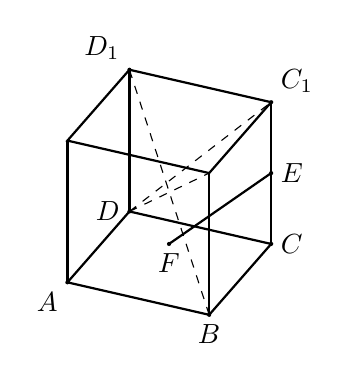
\begin{tikzpicture}[>=stealth,scale=0.75]
  \coordinate (A) at (0,0); \coordinate (B) at (2.4,-0.55);
  \coordinate (C) at (3.45,0.65); \coordinate (D) at (1.05,1.2);
  \coordinate (A1) at (0,2.4); \coordinate (B1) at (2.4,1.85);
  \coordinate (C1) at (3.45,3.05); \coordinate (D1) at (1.05,3.6);
  \coordinate (E) at (3.45,1.85); \coordinate (F) at (1.72,0.65);
  \draw[thick] (A)--(B)--(C)--(D)--cycle;
  \draw[thick] (A1)--(B1)--(C1)--(D1)--cycle;
  \draw[thick] (A)--(A1) (B)--(B1) (C)--(C1) (D)--(D1);
  \draw[dashed] (B)--(D1) (D)--(B1) (D)--(C1);
  \draw[thick] (E)--(F);
  \fill (A) circle (1pt) node[below left] {$A$};
  \fill (B) circle (1pt) node[below] {$B$};
  \fill (C) circle (1pt) node[right] {$C$};
  \fill (D) circle (1pt) node[left] {$D$};
  \fill (D1) circle (1pt) node[above left] {$D_1$};
  \fill (C1) circle (1pt) node[above right] {$C_1$};
  \fill (E) circle (1pt) node[right] {$E$};
  \fill (F) circle (1pt) node[below] {$F$};
\end{tikzpicture}
